\begin{figure}[H]
    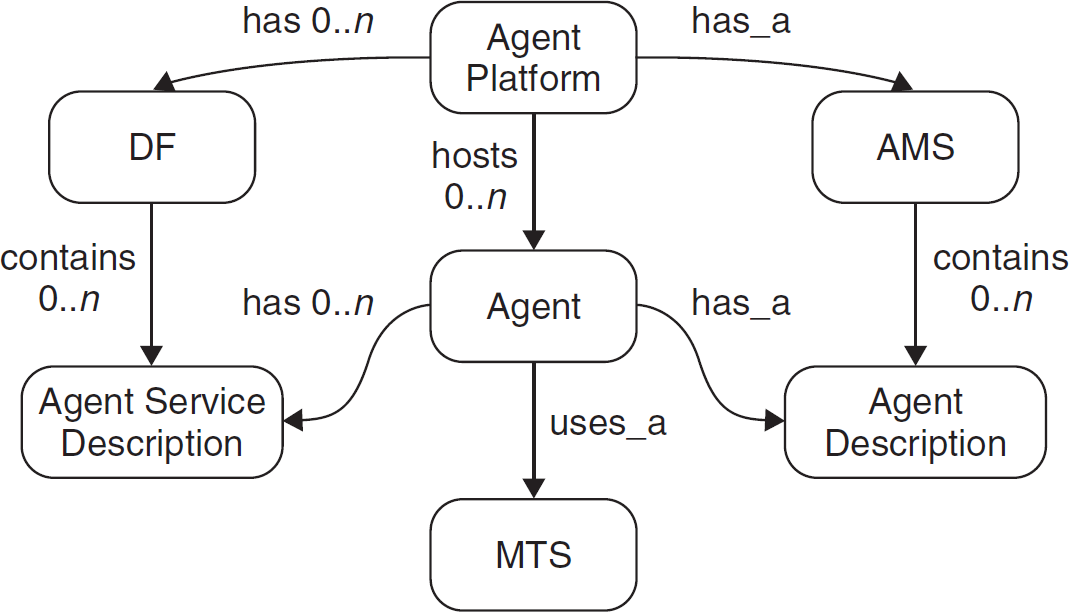
\includegraphics[width=10cm]{images/jade_structure.png}
    \centering
    \caption{\textit{Entity-Relationship}-Diagramm aus \cite{book:jade}}
    \label{fig:jade_structure}
\end{figure}

\paragraph{\textit{Agent Platform} (AP)}
Die AP beschreibt die physikalische Infrastruktur in der die Agenten ausgeführt werden. Hier sind die Rechner, die Netzwerke, die Betriebssysteme, das \textit{Agent Management System}, die Agenten selbst und zusätzliche Software mit inbegriffen.

\paragraph{Agent}
Ein Agent existiert in der AP und bietet ein oder mehrere Services die mit Hilfe einer \textit{Service Description} veröffentlicht sind. Ein Agent hat ein eindeutigen \textit{FIPA Agent Identifier} (AID).  

\paragraph{Diretory Faciliator (DF)}
Der DF ist eine optionale Komponente. Der DF stellt den Agenten einen "'Gelbe Seiten"'-Service zur Verfügung und hält eine komplette Liste aller Agenten. Der "'Gelbe Seiten"'-Service wird von den Agenten genutzt um ihre Services zu registrieren und somit den anderen Agenten verfügbar zu machen. Die AP kann beliebig viele DF starten, die ihre Daten untereinander synchronisieren.

\paragraph{Agent Management System (AMS)}
Das AMS ist für das Erstellen und Löschen der Agenten verantwortlich. Jeder Agent muss sich beim AMS registrieren. Bei diesem Schritt vergibt das AMS dann die AID für die Agenten. Ein Agent beendet sich, wenn er sich vom AMS abmeldet. Das AMS ist als eine Entität zu verstehen und erstreckt sich auch über mehrere Rechner.

\paragraph{Message Transport Service (MTS)} Dieser Service wird von der AP bereitgestellt. Über ihn können die Agenten Nachrichten austauschen.